\documentclass{article}
\usepackage{pgfplots}
\pgfplotsset{compat=1.16}

\begin{document}

\begin{figure}[h]
    \centering
    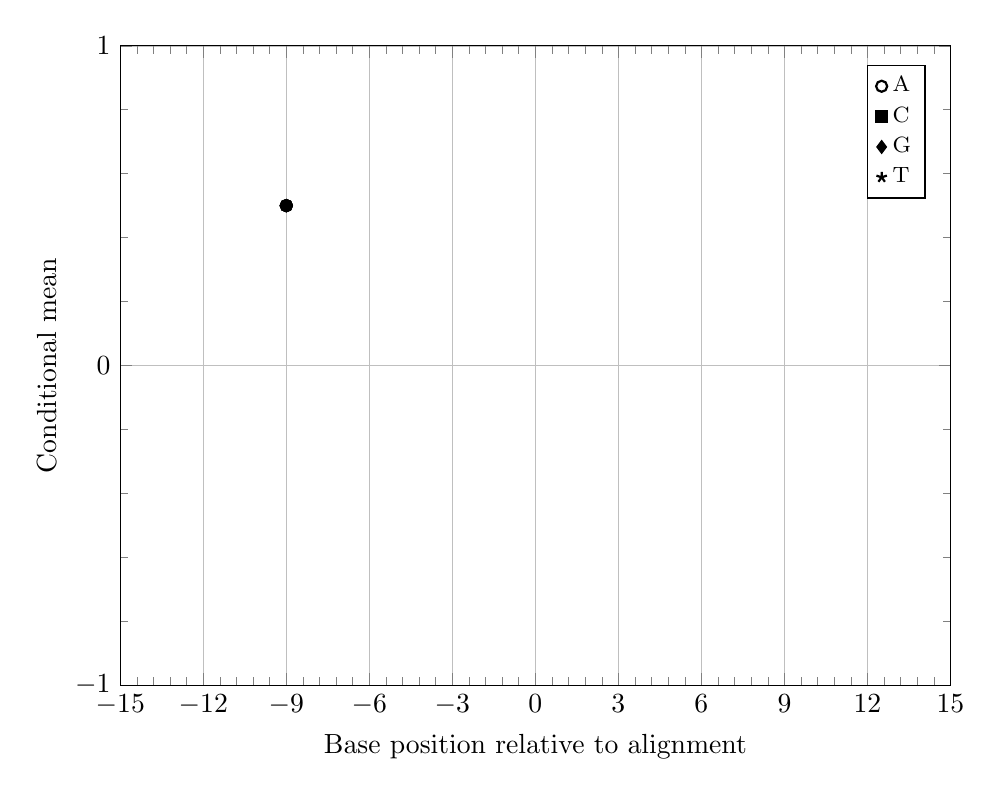
\begin{tikzpicture}
        \begin{axis}[
            width=\textwidth,
            height=0.8*\textwidth,
            xlabel={Base position relative to alignment},
            ylabel={Conditional mean},
            xmin=-15, xmax=15,
            ymin=-1, ymax=1,
            xtick={-15,-12,...,15},
            ytick={-1,0,1},
            grid=major,
            grid style={line width=.1pt, draw=gray!10},
            major grid style={line width=.2pt,draw=gray!50},
            minor tick num=4,
            minor grid style={line width=.1pt,draw=gray!30},
            legend pos=north east,
            legend cell align=left,
            legend style={font=\footnotesize},
            every axis plot/.append style={thick},
            scatter/classes={
                A={mark=o,black},
                C={mark=square*,black},
                G={mark=diamond*,black},
                T={mark=star,black}
            },
            scatter,
            visualization depends on={value \thisrow{label} \as \labelname}
        ]
            \addplot[scatter,only marks] table [x expr=\thisrow{x}, y expr=\thisrow{y}, meta=label] {
                x   y   label
                -9  0.5 A
                -9  0.5 C
                -9  0.5 G
                -9  0.5 T
            };
            \legend{A,C,G,T}
        \end{axis}
    \end{tikzpicture}
    \caption{Mean (normalized) R10 ONT raw signal value conditioned on individual nucleotide base at a given (relative) position. Over a large set of sequences aligned to their respective raw signals, the value on the y-axis is calculated by computing the average signal value overall signal values where a base at a position relative to the aligned base attains the value indicated by the legend. The lighter area indicates the sequence of bases that forms the $10$-mers used in this work. Our $10$-mers extend the $9$-mers used in ONTs Remora toolkit by the leftmost base at relative position $-7$, which allows us to more effectively handle the step-back mechanism described later.}
    \label{fig:conditional_mean}
\end{figure}

\end{document}